%!TEX root = Thesis.tex
\chapter{Implementation and Evaluation}
	The chapter contains practical part of the work, describing implementation of defined in the Chapter 4 modules together with basic content. The prototype implements major aspects proposed in the concept, according to 3-tier architecture. 

	Namely next components:
	 \begin{itemize}
		\item \textbf{Client Tier} presents adaptive to different screens GUI, dynamically changed content and cookies for authorization
		\item \textbf{Application Tier} consists web frameworks for GUI representation and application logic implementation, XMPP server(with protocol extensions) and guarantee appropriate interface of collaboration between tiers via JSON/XML formats
		\item \textbf{Data Tier} consists descriptional metadatadata of sensors and streaming of a map of values, images and text provided by different types of data sources
	\end{itemize}
	To make evaluations real, system will use data from temperature sensor which is provided as a testing environment in scope of ACDSee project, together with TU Dresden, BTU Cottbus - Senftenberg and RWTH Aachen University. It locates in the room INF3084, Faculty of Information Technology, Chair of Computer Science.


\section{Development Environment}
	As a programming languages for implementation of this work jQuery\footnote{jQuery programming language, \url{http://jquery.com/}} and HTML5\footnote{HTML specification, \url{http://www.w3.org/wiki/HTML/Specifications}} together with CSS\footnote{CSS specification, \url{http://www.w3.org/Style/CSS/specs.en.html}} was chosen. jQuery is a fast, small, well documented, easy and widely used and feature-rich JavaScript library. Where the JavaScript is most commonly used as part of web browsers, whose implementations allow client-side scripts to interact with the user, control the browser, communicate asynchronously, and alter the document content that is displayed. It is also being used in server-side programming, game development and the creation of desktop and mobile applications. In addition to JavaScript Jquery has such an important properties as: chaining, easy-to-use AJAX, event handlers, CSS selectors, pluins. It makes things like HTML document traversal and manipulation, event handling, animation, and Ajax much simpler with an easy-to-use API that works across a multitude of browsers. It enables the project code to be portable over different platforms and provides opportunity for robust and effective development. The choice is dictated mostly by two aspects. On the one hand, the system that is being developed is distributed by it's nature. On the other hand, jQuery has low entry barrier, and the code written in this language is extremely readable, laconic and understandable. These facts make further support of written code much easier for other developers that have an experience with any other JavaScript library. 
	\newline
	To show justification of choosen approach was made comprehensive comparison between main web toolkits/libraries as Dojo\footnote{Dojo documentation, \url{http://dojotoolkit.org/features/}}, Prototype\footnote{Prototype documentation, \url{http://prototypejs.org/}}, Yahoo User Interface(YUI) and ExtJS\footnote{ExtJS documentation,\url{http://docs.sencha.com/extjs/4.2.2/}} that shown in the Table 5.1. 
	\begin{table}[H]
	\centering
	\begin{tabular}{|L{3cm}|l|L{2cm}|l|L{2cm}|L{2cm}|}
	\hline
	Target 			& jQuery & Dojo & Prototype & YUI & ExtJS \\
	\hline
	\hline
	License		& MIT & BSD \& AFL & MIT & BSD & GPL and Commercial \\
	\hline
	Size		& 32 KiB & 41 kB & 46–278 kB & 31 kB & 84–502 kB \\
	\hline
	Source language		& JavaScript & JavaScript + HTML & JavaScript &  Javascript + HTML + CSS & JavaScript \\
	\hline
	Grid		& yes & yes & yes & - & yes  \\
	\hline
	DOM wrapped		& yes & yes & yes & no & yes \\
	\hline
	Other data retrieval		& XML, HTML & XML, HTML, CSV, ATOM & - & yes & XML  \\
	\hline
	DOM wrapped		& yes & yes & yes & no & yes \\
	\hline
	Server push data retrieval		& yes & yes & - & via Plugin & yes \\
	\hline
	GUI page layout		& with Plugin & yes & yes & - & yes \\
	\hline 		
	Touch events		& with Plugin & yes & yes & - & yes \\
	\hline 
	\end{tabular}
	\caption[Caption in TOC]{Comparison of JavaScript frameworks}
	\label{tab:JS_frameworks}
	\end{table}
	Also the most important part is a version of browser support which is presented in the Table 5.2 . jQuery\footnote{jQuery browser support, \url{http://jquery.com/browser-support/}}, Dojo\footnote{Dojo browser support,\url{http://livedocs.dojotoolkit.org/releasenotes/1.4}}, Prototype\footnote{Prototype browser support, \url{http://prototypejs.org/doc/latest/Prototype/Browser/index.html}}, YUI\footnote{YUI browser support, \url{http://yuilibrary.com/yui/environments/}}, ExtJS\footnote{ExtJS browser support, \url{http://www.sencha.com/products/extjs/}}.

	\begin{table}[H]
	\centering
	\begin{tabular}{|r|l|l|l|l|l|}
	\hline
	Target 			& jQuery & Dojo & Prototype & YUI & ExtJS \\
	\hline
	\hline
	Chrome		& 1+ & 3 & 1+ & - & 10+ \\
	\hline
	Opera		& 9+ & 10.50+ & 9.25+ & 10.0+ & 11+ \\
	\hline
	Safari		& 3+ & 4 & 2.0.4+ & 4.0 & 4+ \\
	\hline
	Mozilla Firefox		& 2+ & 3+ & 1.5+ & 3+ & 3.6+ \\
	\hline
	Internet Explorer		& 6+ & 6+ & 6+ & 6+ & 6+ \\
	\hline
	\end{tabular}
	\caption[Caption in TOC]{Browser Support}
	\label{tab:internal_results}
	\end{table}
    
    \textbf{XMPP Client on JavaScript}

	Web applications are cross-platform, easily deployable, and come with a large user base already familiar with them. More than that, web technologies make heavy use of HTML, and it is often the case that tools for manipulating HTML work very well on XML, and therefore, on XMPP, which is build based on Jquery. XMPP specification standardized the format of message by using stanzas, which is based on XML format and use XMPP-oriented tags. Thus, in order to implement web-based client-side application based on XMPP was used Strophe.js\footnote{Strophe.js an XMPP library for JavaScript, \url{http://strophe.im/strophejs/}}.

    \textbf{Strophe.js} is a collection of libraries for speaking the XMPP protocol, targeting browser-based clients and available under the MIT license. While most XMPP libraries and implementations are focused on chat-based applications, Strophe.js takes a wider view. It has been used to implement not only traditional messaging applications, but also for real-time games, notification systems and search engines. The implementations are production ready since year 2009, well documented and easy to extend. It uses BOSH, a binding of XMPP to HTTP using long polling and WebSockets, a full-duplex single socket connection to a server. With Strophe.js become possible to interconnect different data types(text, map of values, images, logs nd etc.).

    Strophe.js define and implements main methods and functions to generate, send and transfer XML-based stanzas. Also it has methods which allows to connect to a XMPP server, to send a message to a user, to add a contact - and it knows about the XML that needs to be sent to the server to carry out these actions. 

\section{Web-based Framework Analysis}
 \begin{itemize}
	\item \textbf{Twitter Bootstrap}
	\newline
	Twitter Bootstrap is the most popular and widely used framework, nowadays. It's a beautiful, intuitive and powerful web design kit for creating cross browser, consistent and good looking interfaces. It offers many of the popular UI components with a plain-yet-elegant style, a grid system and JavaScript plugins for common scenarios.

	It consists of four main parts:
	Scaffolding – global styles, responsive 12-column grids and layouts. Has some expressive features like tablets and mobile grids which maintain the grid column structure instead of collapsing the grid columns into individual rows when the viewport is below 768 or 480 pixels wide. Base CSS – this includes fundamental HTML elements like tables, forms, buttons, and images, styled and enhanced with extensible classes. Components – collection of reusable components like dropdowns, button groups, navigation controls (tabs, pills, lists, breadcrumbs, pagination), thumbnails, progress bars, media objects, and more. JavaScript – jQuery plugins which bring the above components to life, plus transitions, modals, tool tips, popovers, scrollspy (for automatically updating nav targets based on scroll position), carousel, typeahead (a fast and fully-featured autocomplete library), affix navigation, and more. Twitter Bootstrap in addition to vanilla CSS includes support for the two most popular preprocessors, Less and Sass.
	
	\item \textbf{Foundation}
	\newline
	Foundation is a powerful, feature-rich, responsive front-end framework. With Foundation user can quickly prototype and build websites or apps that work on any kind of device, with tons of included layout constructs, elements and best practices. It's built with mobile first in mind, utilitizes semantic features, and uses Zepto instead of jQuery in order to brings better user experience and faster performance.

	Foundation has a 12-column flexible, nestable grid powerful enough to create rapidly multi-device layouts. There are styles for typography, buttons, forms, and various navigation controls. And, JavaScript plugins including dropdowns, orbit (a responsive image slider with touch support), reveal(for creating modal dialogues or pop-up windows) and tooltips.
	
	\item \textbf{GroundworkCSS}
	\newline
	GroundworkCSS is a new, fresh addition to the front-end frameworks family. It's a fully responsive HTML5, CSS and JavaScript toolkit built with the power of Sass and Compass which gives the ability to rapidly prototype and build websites and apps that work on virtually any device.

	It offers an flexible and fluid grid system that makes creating any layout possible. Feature is a jQuery ResponsiveText plugin which allows to have dynamically sized text that adapts to the width of the viewport: extremely useful for scalable headlines and building responsive tables. The framework includes UI components like tabs, responsive data tables, buttons, forms, responsive navigation controls, tooltips, modals and many more. It also offers a set of vector social icons and a full suite of pictographic icons included in FontAwesome. GroundworkCSS is well documented with many examples. The only thing as a weakness is the missing of a way to customize download.

	\item \textbf{Gumby}            
	\newline
	Gumby is simple, flexible, and robust front-end framework built with Sass and Compass.
 
	Its fluid-fixed layout self-optimizes the content for desktop and mobile resolutions. It supports multiple types of grids, including nested ones, with different column variations. Gumby has two PSD templates that get user started designing on 12 and 16 column grid systems. The framework offers feature-rich UI Kit which includes buttons, forms, mobile navigation, tabs, skip links, toggles and switches, drawers, responsive images, retina images, and more. An awesome set of responsive, resolution independent Entypo icons, is completely integrated into the Gumby Framework. Gumby has also a good customization. 
	
	\item \textbf{Kube}
	\newline
    Kube is a minimal, responsive and adaptive framework with no imposed styling which gives to user the freedom to create. It offers basic styles for grids, forms, typography, tables, buttons, navigation, and other stuff like links or images. The framework contains one compact CSS file for building responsive layouts with ease and two JS files for implementing tabs and buttons in your designs. If user is looking for maximum flexibility and customization, user can download developer version which includes LESS files, with variables, mixins and modules.
	\end{itemize}

	\begin{figure}[!ht]
	\centering
	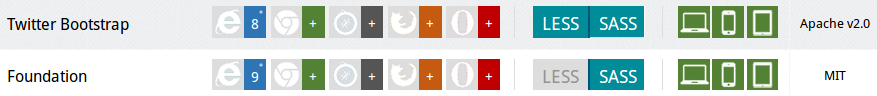
\includegraphics[scale=0.7]{images/Bootstrap&Foundation.png}
	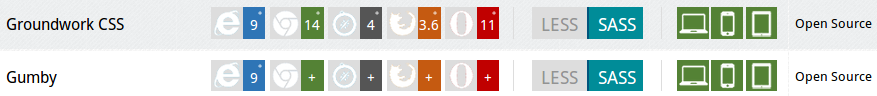
\includegraphics[scale=0.7]{images/Groundwork&Gumby.png} 
	
\includegraphics[scale=0.7]{images/Kube.png}  
	\caption[Framework Comparison]{Framework Comparison\footnote{\url{http://usablica.github.io/front-end-frameworks/compare.html}}}
	\label{img:Bootstrap&Foundation.png}
	\label{img:Groundwork&Gumby.png}   
	\label{img:Kube.png}                          
	\end{figure}

 Among all of the described above Web frameworks the most reasonable to choose Twitter Bootstrap. It has all possible nowadays visualization modules, have been used for more than 1500+ sites, well-known among developers, reach API and examples, supported by all browsers, has a build-in fluid grid systems, customizable, that is simplify a lot development of a cross-browser application.

 Examples of used modules of a Twitter Bootstrap are shown on a screenshots in the section 5.7. It consists: buttons, navigation tabs bar, log in form, search field, 4/3/2-columns  grid layout, modals, tooltips and carousel for preview images. All GUI was made by using only CSS and HTML structure of a Twitter Bootstrap. All animations, appearence, dynamic adaptivity was done by using special tags, anchors and classes. 

\section{JavaScript MV* Frameworks}
	As was mentioned in the section 4.3.3, very important to realize loosely coupled system. Needs to be separated visualization of graphical modules on a web page from a code that is responsible for retrieving of a content. Thus was used AngularJS\footnote{AngularJS,\url{http://angularjs.org/}}. It is an open-source JavaScript framework, maintained by Google, that assists with running single-page applications. Its goal is to augment web-based applications with model–view–controller (MVC) capability, in an effort to make both development and testing simpler.The library reads in HTML that contains additional custom tag attributes; it then obeys the directives in those custom attributes, and binds input or output parts of the page to a model represented by standard JavaScript variables. The values of those JavaScript variables can be manually set, or retrieved from static or dynamic JSON resources\cite{ wiki:angular}. AngularJS is a toolset for building the framework most suited to application development. It is fully extensible and works well with other libraries such as jQuery, on top of which was build XMPP. Every feature can be modified or replaced to suit unique development workflow and feature needs.

    The framework adapts and extends traditional HTML to better serve dynamic content through two-way data-binding(Figure 5.2) that allows automatic synchronization of models and views. As a result, AngularJS deemphasizes DOM manipulation and improves testability.

	\emph{Design goals}:
	\newline
	Decouple DOM manipulation from application logic. This improves the testability of the code. Decouple the client side of an application from the server side. This allows development work to progress in parallel, and allows for reuse of both sides.	Angular follows the MVC pattern of software engineering and encourages loose coupling between presentation, data, and logic components. Using dependency injection, Angular brings traditional server-side services, such as view-dependent controllers, to client-side web applications. Consequently, much of the overheads on the backend is reduced, leading to much lighter web applications.

   \emph{Two-way data binding}
        \begin{figure}[!ht]
		\centering
		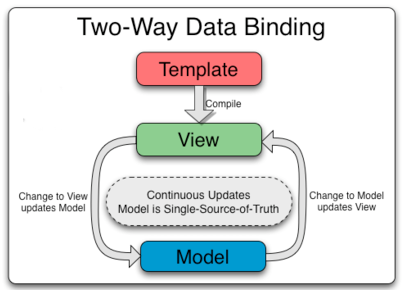
\includegraphics[scale=0.8]{images/2wayBinding.png}   
		\caption[Two-way data binding]{Two-way data binding\footnote{Angular JS Two-Way Data Binding,\url{http://docs.angularjs.org/guide/databinding}}}                         
		\end{figure}
	AngularJS two-way data binding is a most notable feature and reduces the amount of code written by relieving the server backend from templating responsibilities. Instead, templates are rendered in plain HTML according to data contained in a scope defined in the model. The \$scope service in Angular detects changes to the model section and modifies HTML expressions in the view via a controller. Likewise, any alterations to the view are reflected in the model. This circumvents the need to actively manipulate the DOM and encourages bootstrapping and rapid prototyping of web applications.

	The way Angular templates works is different, as illustrated on the Figure 5.3. They are different because first the template (which is the uncompiled HTML along with any additional markup or directives) is compiled on the browser, and second, the compilation step produces a live view. Any changes to the view are immediately reflected in the model, and any changes in the model are propagated to the view. This makes the model always the single-source-of-truth for the application state, greatly simplifying the programming model for the developer. View in such a way simply an instant projection of a model.
	    \begin{figure}[!ht]
		\centering
		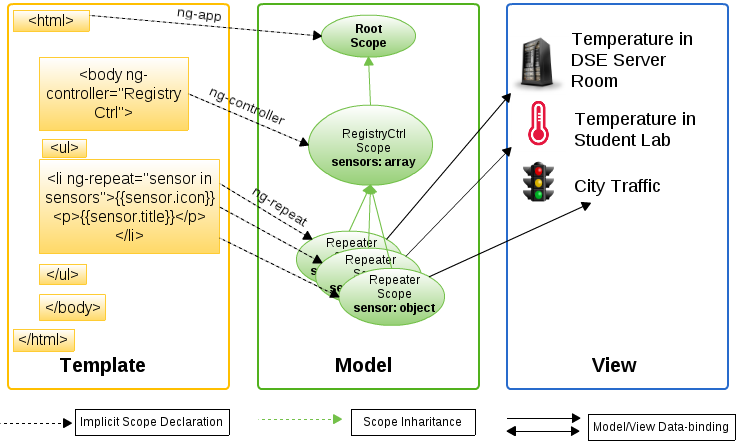
\includegraphics[scale=0.6]{images/3wayBinding.png}   
		\caption[Template Model View]{Template Model View}                         
		\end{figure}
        
    Because the view is just a projection of the model, the controller is completely separated from the view and unaware of it. As shown on the figure above, the resulting view can be applied to every data available on a backend. Model handler automaticaly generates a view for every new sensor. No need to change code or add new id and dependent handlers, variables, channels. 
    
    The template declaire the structure of what have to be shown on user view, which is generated on a Web Server. Model repeats to generate the same view of every sensor in the list, which is coming from a controller as parameter {{sensor}} with possible attributes {{sensor.icon}} and {{sensor.titel}}, till the list of registered sensors will be finished.

    The code realization of such a flow are shown on the Listing~\ref{angular_template}
    \begin{lstlisting}[label=angular_template,caption=Template registry.html]
<div id="sensor_list">
    <div class="grid-sizer"></div>
    <div class="masonry-brick sensor-wrapper" id="{{sensor.id}}" ng-repeat="sensor in sensors | filter:{title: query}">
        <div class="sensor" ng-controller="RegistryCtrl" ng-click="open()">
            <div class="icon">
                <img class="img-responsive" ng-src="{{sensor.icon}}">
                <h4>{{sensor.title}}</h4>
                <span class="label label-success" ng-show="user.check_subscribe(sensor.id)">Subscribed</span>
            </div>
            <div ng-show="sensor.picture">
                <img class="img-responsive" ng-src="{{sensor.picture}}">
            </div>
            <span class="description">{{sensor.description}}</span>
        </div>
    </div>
</div>
    \end{lstlisting}
    Model explicitly integrated to the HTML, as shown on the Listing 5.1 by using directive injection: ng-repeat, ng-src, ng-click and also variables {{sensor.*}}. On the Listing~\ref{angular_controller} shown the controller "RegistryCtrl" implementation.

    \begin{lstlisting}[label=angular_controller,caption=Controller controller.js]
var sensdash_controllers = angular.module("sensdash.controllers", []);

sensdash_controllers.controller("RegistryCtrl", ["$scope", "Registry", "User",
    function ($scope, Registry, User) {
        Registry.load().then(function(sensors){
            $scope.sensors = sensors;
        });
        $scope.user = User;
    }]);
    \end{lstlisting}

	On the listing~\ref{angular_service} factory service, module of the AngularJS, parses Web API and creates sensors array based on a factory pattern. The main goal of this pattern to create an object, independently from it's type. This pattern applied to every data source. Such type of loose coupling helps to avoid code dublication, overhead and simplify code maintenance.  

    \begin{lstlisting}[label=angular_service,caption=Controller controller.js]
var sensdash_services = angular.module('sensdash.services', ['ngResource']);

sensdash_services.factory('Sensor', ['$resource',
    function ($resource) {
        return $resource('api/sensors/:sensorId', {}, {
            query: {method: 'GET', params: {sensorId: 'all'}, isArray: true}
        });
    }]);
    \end{lstlisting}


\section{Interface Implementation}
	 According to system architecture system has to implement two main types of intefaces:
	 \begin{itemize}
	 \item Registry-Directory Manager
	 \item Data Hub-DataStream Handler and AuthHandler
	 \end{itemize}
	 XMPP connections live for arbitrarily long periods of time, but HTTP requests are quite short lived.
	A DataStream Manager maintains an XMPP connection for a third party and provides access to the connection via the HTTP long polling technique.
	    \begin{figure}[!ht]
		\centering
		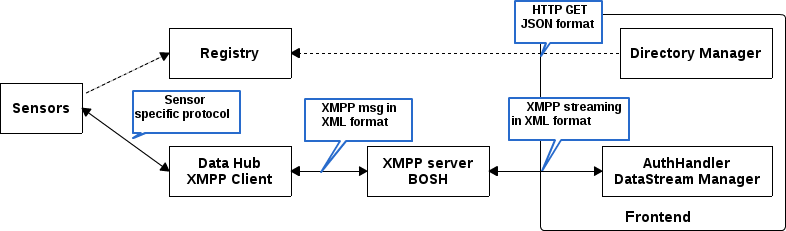
\includegraphics[scale=0.6]{images/XMPPflow.png}   
		\caption[XMPP BOSH/Stream]{XMPP interface flow}                      
		\end{figure}

	The browser and the DataStream Manager communicate over HTTP using a Bidirectional-streams Over Synchronous HTTP(BOSH). Essentially, BOSH helps an HTTP client establish a new XMPP session, then transports stanzas back and forth over HTTP wrapped in a special <body> element. It also provides some security features to make sure that XMPP sessions can't be easily hijacked. The DataStream Manager communicates with the XMPP server as if it were a normal client. In this way, an HTTP application can control a real XMPP session. Because of the efficiency and low latency afforded by the long polling technique, the end result competes with native connections.

	XMPP connections are managed through the Strophe.Connection object. DataStream Manager which includes BOSH connection managers are exposed to HTTP clients as URLs, and the Strophe.Connection object needs to know about one of these URLs. Many XMPP servers come with support for BOSH built in, and they typically expose the service at http://example.com:5280/http-bind or http://example.com:5280/xmpp-httpbind.

	It may seem like a lot of effort to get XMPP into a browser, but not only does this work well in practice, it turns out this technique even has some advantages over direct XMPP connections:
	\begin{itemize}
	\item Interactions with the connection manager are request by request, which allows the client to move from network to network. The managed connection stays available even if the end user's IP address changes several times.
	\item Because one failing request doesn't terminate the managed connection, these managed sessions are extremely robust and tolerant of temporary network failure.
	\item Because connection managers cache and resend data for a request, no needs to worry about losing data when connection is interrupted.
	\item HTTP is extremely firewall friendly, and because most connection managers run on standard HTTP ports, managed connections still work even in limited network environments that don’t allow anything but HTTP.
	\end{itemize}

	To create a new Strophe.Connection object used the new keyword~\ref{js_object}.	Once a connection object was created, calls connect() and disconnect() can be used to start and end	communication with the server:
	    \begin{lstlisting}[label=js_object,caption=Stanzas Format]
		var conn = new Strophe.Connection("http://example.com:5280/xmpp-httpbind");
		// starting a connection to example.com
		conn.connect("user@example.com", "mypassword", my_callback);
		// disconnecting
		conn.disconnect();
	    \end{lstlisting}
	The first two parameters to connect() are the JID and password to use to authenticate the session, and the last parameter is the callback function. The callback function will be called with a single parameter that is set to one of the statuses (CONNECTED, DISCONNECTED, AUTHFAIL, CONNFAIL and etc.). A simple callback function that disconnects once the connection reaches the CONNECTED phase is shown here: 
	\begin{lstlisting}[label=js_object,caption=Stanzas Format]
		function my_callback(status) {
		if (status === Strophe.Status.CONNECTED) {
		 conn.disconnect();
		 }
	    }
	\end{lstlisting}
Every time the connection changes its status, this callback function is executed. The callback function simply ignores any status but the CONNECTED status, and disconnects once the connection has reached that status.

\textbf{Mechanism of Sessions}
\newline
XMPP is a TCP-based protocol, just like HTTP, and communication happens over an established, mostly reliable socket between two endpoints. The BOSH extension to XMPP provides a bridge between this bidirectional, stateful protocol and HTTP, which is unidirectional and stateless. Because a web browser cannot directly connect to an XMPP server, a BOSH connection manager responds to requests from a browser using HTTP and uses them to manage an XMPP connection on behalf of the user(Figure 5.5).  XMPP's basic model of communication is Client -> Server -> Server -> Client, and in support of this it defines a Client to Server protocol and a Server to Server protocol.
  \begin{figure}[!ht]
  \centering
  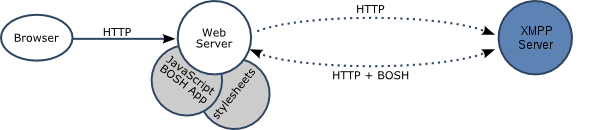
\includegraphics[scale=0.6]{images/xmpp-bosh.png}   
  \caption[BOSH]{XMPP BOSH}                         
  \end{figure} 

Aside from the socket needed for XMPP communication, each managed connection has two other pieces of data associated with it: the session identifier(SID) and the request identifier(RID). SID stands for Session Identifier. This uniquely identifies the managed XMPP connection, and it is often a long, opaque alphanumeric string. Even though it is enough to identify the session, it is not very useful on its own. The RID identifies a particular HTTP request associated with a BOSH-managed connection. Before a connection is established, the client sends a random RID to the DataStream Manager along with its first request. Each subsequent request increments the RID by one. The SID and the RID together provide enough information to interact with the underlying XMPP connection. Because the RID is generated randomly from a very large range of numbers, it is virtually impossible to guess the RID. Also, the DataStream Manager will reject RIDs that fall outside of a narrow window around the current request. In this way, the BOSH-managed connection is tolerant of small errors like out of order delivery but robust to attacks like hijacking the connection. Because these two identifiers are enough to both address and make use of a managed XMPP session, if an application knows the SID and the RID, it can take over or attach to the underlying session.

The attach() function demonstrats sending SID and RID through a BOSH connection in the Listing~\ref{BOSH_callback}):
	    \begin{lstlisting}[label=BOSH_callback,caption=BOSH Callback]
		var connection = new Strophe.Connection(BOSH_URL);
        connection.attach(jid, sid, rid, callback);
	    \end{lstlisting}

BOSH sessions can be encrypted, and often the underlying XMPP sessions are encrypted as well. Because XMPP makes use of SASL, the authentication mechanisms tend to be quite strong.

\subsection{XEP-0045: Multi-User Chat}
Traditionally, instant messaging is thought to consist of one-to-one chat rather than many-to-many chat, which is called variously "groupchat" or "text conferencing". The Jabber/XMPP community developed and implemented a basic groupchat protocol since 1999. That "groupchat 1.0" (GC) protocol provided a minimal feature set for chat rooms but was rather limited in scope. The Multi-User Chat or MUC builds on the older groupchat 1.0 protocol in a backwards-compatible manner but provides advanced features such as invitations, message presence, room moderation and administration, and specialized room types\footnote{XEP0045, \url{http://xmpp.org/extensions/xep-0045.html}}.

\subsubsection{Requirements}
In scope of this master thesis can be addressed only the minimal functionality provided by Jabber-based multi-user chat services that existed in 2002 when development of MUC began. Builded on top of groupchat 1.0 protocol. 

Each room is identified as a "room JID" <room@service> (e.g., <jdev@conference.jabber.org>), where "room" is the name of the room and "service" is the hostname at which the multi-user chat service is running. Each occupant in a room is identified as an "occupant JID" <room@service/nick>, where "nick" is the room nickname of the occupant as specified on entering the room or subsequently changed during the occupant's visit. A user enters a room (i.e., becomes an occupant) by sending directed presence to <room@service/nick>. An occupant can change his or her room nickname and availability status within the room by sending presence information to <room@service/newnick>. Messages sent within multi-user chat rooms are of a special type "groupchat" and are addressed to the room itself (room@service), then reflected to all occupants. An occupant exits a room by sending presence of type "unavailable" to its current <room@service/nick>.
The coommon system architecture has the next structure(Figure ):
  \begin{figure}[!ht]
		\centering
		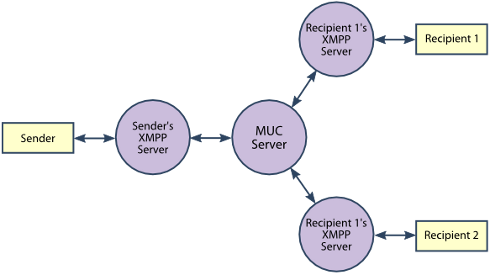
\includegraphics[scale=0.8]{images/MUC.png}   
		\caption[MUC]{MUC System Architecture}                         
		\end{figure}

\textbf{Public Speaking}
\newline
Group chat allows multiple people to gather in the same place to discuss a topic. These virtual meeting places are called rooms. Rooms can have access controls, moderators, administrators, and even automatic logging and archival of the group’s communications.
\emph{Group Chat Services}
\newline
Group chat is provided as a service, usually alongside a regular XMPP server. The group chat service has its own domain; for example, the jabber.org server runs a group chat service at conference.jabber.org. Each room on the group chat service gets its own address, which looks just like a user’s JID. General XMPP-related chat takes place in jabber@conference.jabber.org.

\emph{Entering and Leaving a Room}
Before making any changes in a chat room a user have to enter the room. This is also often referred to as joining the room. After a user done, he/she leaves the room. Because this mirrors the concept of a user coming and going on and offline, the multi-user chat designers decided to model this part of the protocol with <presence> stanzas. Users can join a group chat room by sending available presence to the room, along with a note that they understand the multi-user chat protocol. Sending presence directly to a JID instead of to the user’s server is called directed presence. Similarly, to leave, unavailable presence is sent to the room. Sending presence stanzas directly to a JID instead of to the user’s server is called sending directed presence.

If Jane wants to join the group chat room for the Temperature sensor, they will both need to send directed presence to their desired identity in the room temperature@chat.sensor.lit. Their stanzas are shown in the Listing~\ref{stanzas_muc}:
\begin{lstlisting}[label=stanzas_muc,caption=Stanzas Format for MUC]
<presence to="temperature@chat.sensor.lit/jane"
          from="jane@example.lit/sensor">
    <x xmlns="http://jabber.org/protocol/muc"/>
</presence>
\end{lstlisting}

Once they have joined the room, the group chat service will broadcast all the other participants' presence statuses to them. After all the other participants’ presence stanzas are sent, the server concludes the presence broadcast by sending the arriving participant’s presence to everyone, including the new arrival. Thus, when a new participant sees their own presence broadcast back to them, they know they have fully joined the room.

The room sends the affiliations and roles of each participant along with their presence. Jane's own presence broadcast also includes a status code of 110, which signals that this presence refers to the user herself. Just as with presence updates from Jane’s roster, Jane will also receive presence updates from the room as people leave and new people join on the listing~\ref{muc_affiliation}.
\begin{lstlisting}[label=muc_affiliation,caption=Server Presence Notification]
<presence to="jane@example.lit/sensor"
          from="temperature@chat.sensor.lit/jane">
  <x xmlns="http://jabber.org/protocol/muc">
      <item affiliation="member" role="participant"/>
      <status code="110"/>
  </x>
</presence>
\end{lstlisting}

\textbf{Creating Rooms}
Thousands of rooms in the federated XMPP network are already available to participate in, but sometimes room not yet exist. Creating rooms is accomplished in much the same manner as joining a room. Actually, rooms can be created just by joining a non-existent room. Assuming the service allows the user to create new rooms, sending directed presence to the desired room JID of the new room will cause the room to be created and the user to be set as the room’s owner. On the Listing~\ref{room_creation}, Mark creates a new room for the News feed:
	\begin{lstlisting}[label=room_creation,caption=MUC Room Creation]
<presence to="chatter@chat.news.lit/mark"
          from="maek@news.lit/drawing_room">
    <x xmlns="http://jabber.org/protocol/muc"/>
</presence>
	\end{lstlisting}

The chat.news.lit service responds with the presence broadcast for the room’s new and only occupant(Listing~\ref{server_respond}):
	\begin{lstlisting}[label=server_respond,caption=Server Respond to Room Creation]
<presence to="mark@news.lit/drawing_room"
          from="chatter@chat.news.lit/mark">
    <x xmlns="http://jabber.org/protocol/muc">
        <item affiliation="owner" role="moderator"/>
        <status code="110"/>
        <status code="20"/>
    </x>
</presence>
		\end{lstlisting}

Mark has the owner affiliation and the moderator role. These attributes give Mark special powers within the room. The 110 status code is sent, just as it was before, and a new status code of 201 is sent, it signals that a new room has been created. More comprehensive information about roles, affiliations, erros and etc can be found in the book\cite{XMPPbook}.

\subsection{XEP-0060: Publish-Subscribe}
Publish-subscribe systems are everywhere: newspapers, blogs, television, and even e-mail lists. There is a channel of communication, subscribers who are interested in data sent on that channel, and publishers who can send data across the channel. The first thing an application must do for a would-be presenter is to create a channel for them to publish sketches. In XMPP pubsub these channels are called \emph{nodes}. The protocol enables XMPP entities to create nodes (services) at a pubsub service and publish information at those nodes; an event notification (with or without payload) is then broadcasted to all entities that have subscribed to the node. Pubsub therefore adheres to the classic Observer design pattern and can serve as the foundation for a wide variety of applications, including news feeds, content syndication, rich presence, geolocation, workflow systems, network management systems, and any other application that requires event notifications\footnote{XEP-0049: Publish-Subscribe, \url{http://xmpp.org/extensions/xep-0060.html}}.

	\textbf{Creating Node}
	\newline
	A pubsub node is created by sending an IQ-set stanza to the pubsub service(Listing~\ref{node_creation}). Where User\_1 creates node "sensor\_data" within "pubsub.sensor1.lit" XMPP host server.
		\begin{lstlisting}[label=node_creation,caption=PubSub Node Creation]
	<iq to="pubsub.sensor1.lit"
	    from="user_1@sensor1.lit/sensor_registry"
	    type="set"
	    id="create1">
	  <pubsub xmlns="http://jabber.org/protocol/pubsub">
	      <create node="sensor_data"/>
	  </pubsub>
	</iq>
		\end{lstlisting}
	Most actions on pubsub nodes will look very similar to this one, the difference between MUC and PubSub stanzas is the <pubsub> element. Pubsub nodes and their configuration are necessary and useful, but they don't do much by themselves. The real value of pubsub nodes is in the events that are published to them and broadcast to subscribers. Anything can be included in a pubsub event. The pubsub service doesn’t know or care what is inside the event; it simply broadcasts this data to a node’s subscribers.

\textbf{Retrieving Item}
User\_2 just subscribed to user\_1's sensor\_data node, and has missed his event broadcasts from earlier in the week.  User\_1 configured his node to persist items and anyone can query his/her node for the most recently published items. Here, user\_2 requests the last five items by sending an IQ-get stanza to the node with the <items> action(Listing 5.12):
\begin{lstlisting}[label=node_creation_example,caption=PubSub Node Creation]
<iq from="user2@longbourn.lit/outside"
    to="pubsub.sensor1.lit"
    type="get"
    id="items1">
  <pubsub xmlns="http://jabber.org/protocol/pubsub">
    <items node="sensor_data" max_items="5"/>
  </pubsub>
</iq>
\end{lstlisting}
The <items> element contains a node attribute just like the other actions. User\_2 has also set the max\_items attribute to 5 because she/he is only interested in the recent history. If she/he had omitted max\_items, the server would interpret it as a request to send all the historical data it has been configured to keep. If she/he had set max\_items to 500, which is much larger than the configured maximum for the node, the server would have sent as many as were available.

\subsubsection{Overview}
The XMPP publish-subscribe extension provides a framework for a wide variety of applications, including news feeds, content syndication, extended presence, geolocation, avatar management, shared bookmarks, auction and trading systems, workflow systems, network management systems, profile management, and any other application that requires event notifications.
\begin{figure}[!ht]
    \centering
    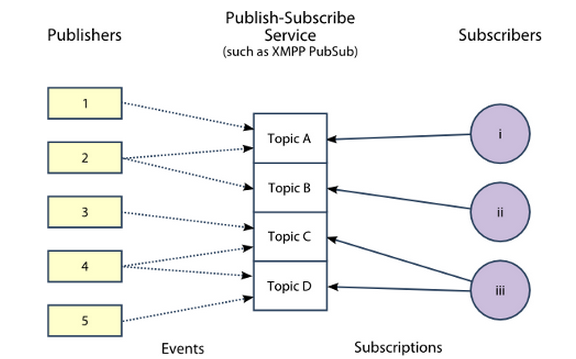
\includegraphics[scale=0.5]{images/XEP0049.png}   
    \caption[General Event Subscription]{General Event Subscription}                      
    \end{figure}

This technology uses the classic "publish-subscribe" or "observer" design pattern: a person or application publishes information, and an event notification (with or without payload) is broadcasted to all authorized subscribers. In general, the relationship between the publisher and subscriber is mediated by a service that receives publication requests, broadcasts event notifications to subscribers, and enables privileged entities to manage lists of people or applications that are authorized to publish or subscribe. The focal point for publication and subscription is a "node" to which publishers send data and from which subscribers receive event notifications. Nodes can also maintain a history of events and provide other services that supplement the pure pubsub model(Figure 5.7)


\subsubsection{Data Flow}
Figure 5.8 shows the process flow of how and when a client can subscribe/retrieve data from a publisher of service through the XMPP PubSub approach. The first thing the DataSource 1 and 2 must do for a would-be presenter is to create a channel for them to publish data - nodes. Once a node is created and configured, Publishers can start send data. Once these events are published, pubsub takes over and makes sure that they get delivered to the subscribed users. In case Publishers want to get a list of their subscribers, it can be retrieved from the pubsub node so that it can present this data to them. If Publisher will become offline its <presence> will be changed automatically to "unavailable" and next time, becoming online and sending new data, all subscribers will receive this information immediately.
    \begin{figure}[!ht]
    \centering
    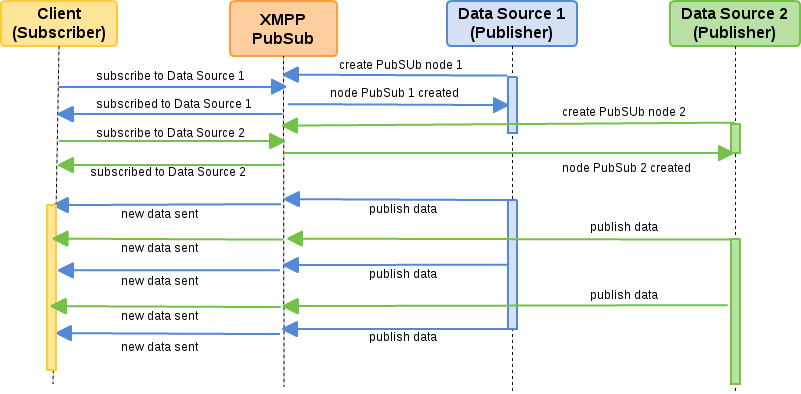
\includegraphics[scale=0.6]{images/PubSub.png}   
    \caption[Service PubSub]{Service PubSub}
    \label{img:pub_sub}                           
    \end{figure}

	\subsubsection{XMPP Stanzas}
	Work is accomplished in XMPP by the sending and receiving of XMPP stanzas over an XMPP stream. Three basic stanzas make up the core XMPP toolset. These stanzas are <presence>, <message>, and <iq>. Each type of stanza has its place and purpose, and by composing the right kinds of quantities of these stanzas, sophisticated behaviors can be achieved. An XMPP stream is a set of two XML documents, one for each direction of communication. These documents have a root <stream:stream> element. The children of this <stream:stream> element consist of routable stanzas and stream related top-level children. Each stanza is an XML element, including its children. The end points of XMPP communication process input and generate output on a stanza-by-stanza basis. The following example shows a simplified and short XMPP session on the Listing~\ref{stanzas}
		\begin{lstlisting}[label=stanzas,caption=Stanzas Format]
		<stream:stream>
			<iq type="get">
				<query xmlns="jabber:iq:roster"/>
			</iq>
			<presence/>

			<message to="darcy@pemberley.lit"
					 from="elizabaeth@longbourn.lit/chatroom"
			         type="chat">
			    <body>Hello chat room</body>
			</message> 

			<presence type="unavailable"/>
		</stream:stream>
		\end{lstlisting}

	In this example, Elizabeth created an XMPP stream by sending the opening <stream:stream> tag. With the stream open, she sents her first stanza, an <iq> element. This <iq> element requested Elizabeth’s roster, the list of all her stored contacts. Next, she notified the server that she was online and available with a <presence> stanza. After noticing that Mr. Darcy was online, she sent him a short <message> stanza. Finally, Elizabeth sent another <presence> stanza to inform the server she was unavailable and closed the <stream:stream> element, ending the session.
    
    \subsubsection{Server}
	The set of XMPP servers that can mutually communicate forms an XMPP network. The set of public XMPP servers forms the global, federated XMPP network. If a server does not speak the server-to-server protocol, it becomes an island, unable to communicate with external servers. An XMPP server will usually allow users to connect to it. It is, however, also possible to write applications or services that speak the server-to-server protocol directly in order to improve efficiency by eliminating routing overhead. Anyone can run an XMPP server, and full-featured servers are available for nearly every platform. Ejabberd, Openfire, and Tigase are three popular open source choices that will work on Windows, Mac OS X, or Linux systems. Several commercial XMPP servers are available as well, including M-Link and Jabber XCP.
	
	\subsubsection{Connection}
	Before any stanzas are sent, an XMPP stream is necessary. Before an XMPP stream can exist, a connection must be made to an XMPP server. XMPP includes some sophisticated support for establishing connections to the right servers. Typically clients and servers utilize the domain name system (DNS) to resolve a server's domain name into an address they can connect to. Email services in particular use mail exchange (MX) records to provide a list of servers that handle mail for a given domain so that one well-known server address does not have to handle every service. Email, being an early Internet application, got special treatment in DNS. These days, service records (SRV) are used to provide a similar function for arbitrary services. The first thing an XMPP client or server does when connecting to another XMPP server is to query the appropriate SRV record at the server’s domain. The response may include multiple SRV records, which can be used to load balance connections across multiple servers. If an appropriate SRV record cannot be found, the application tries to connect to the given domain directly as a fallback. Most libraries also allow you to specify a server to connect explicitly.

	\subsubsection{Long Polling}
	Even with AJAX, data was still being requested, or polled, at timed intervals. Servers can be crippled if too many clients poll too fast.However, to get quick updates, the polling interval needs to be quite small; the lowest latency possible is the length of the polling interval. Another issue with polling is that most poll requests do not receive new data. In order to see changes within a reasonable time frame of when they occur, the polling interval must be quite short, but the actual data may not change very often.	For example, if there is new data ready on the server, the server answers immediately. If there is not new data, the server keeps the connection open, holding any reply. Once new data arrives, it finally responds to the request. If no new data arrives after some period of time, the server can send back an empty reply, so as not to hold too many open connections at once. Once a request is returned, the client immediately sends a new one, and the whole process starts over. Because each polling request is potentially open for a long period of time, this technique is called long polling. It has many advantages over normal polling.
    
    \subsection{PubSub vs MUC}
	\textbf{Pubsub Advantages}
	\newline
	Publish-subscribe is a very generic system, used by many different kinds of applications. The XMPP pubsub extension is similarly generic and is usable for a wide variety of purposes. It assumes nothing about the subscribers; they may be human, or they may be machines. Pubsub nodes, unlike multi-user chat rooms, are arranged in a tree-based hierarchy. This shape is often a more close match to a given problem domain. One of the benefits of the tree shape is that entities can subscribe to non-leaf nodes of the tree, and events published below that node can also be received. Events can be published as notifications or as full payloads, and the subscriber can choose which is most appropriate. Retrieval of the publishing history is built in and fairly fine grained. The subscriber has more fine grained control over the delivery destination. 

	\textbf{Pubsub Disadvantages}
	\newline
	Pubsub, by being so generic, is not optimized for specialized cases. The pubsub extension is not nearly as old or as widely implemented as MUC, and the support for features in both clients and servers varies in quality and depth. Unlike MUC, it is not yet clear what the most used features are, so one must shop around a bit when an advanced feature is needed. There is no special handling of presence built in. There are a few proposed extensions to pubsub that may change this. For example, it would sometimes be useful to limit delivery to available resources only. Tooling for pubsub node creation and configuration is lacking. MUC room creation and configuration is built in to most XMPP clients already. Pubsub has not built-in mechanism for subscribers to interact or find each other. 

	\textbf{Multi-User Chat Advantages}
	\newline
	Presence handling is built in to MUC at a low level. Presence is used to signal joining and leaving of room, and presence changes can also be shared with occupants of the room. MUC is optimized for chat-related use cases and builds on the decades of experience of previous chat systems, especially IRC. All the common moderation and administration features necessary in a collaborative environment are supported - kicking, banning, and various privilege levels. MUC already has many implementations, both of clients and of servers. It is one of the oldest XMPP extensions, and as such, is quite mature and robust. Occupants in MUC rooms can interact with each other, and MUC allows for multiple levels of anonymity to be used as well as private communication.

	\textbf{Multi-User Chat Disadvantages}
	\newline
	Groups of people chatting is the bread and butter of MUC, and MUC is highly optimized for this use case. For example, most MUC servers will automatically send conversation history to every new occupant and generate human-readable messages for most administrative actions. It's possible, and common, to have bots as room occupants, but the experience is designed for human consumption. There is no way to organize chat rooms except as a flat hierarchy, and there is no way to share configurations or participation across collections of rooms. The one exception to this is that most servers have a default configuration that is applied to all rooms on the server. All of these extra human-focused features and administration capabilities make implementation more difficult. Unlike pubsub, MUC implementations have a lot of edge cases to account for in order to be user friendly and robust.


\subsection{XEP-0049: Private XML Storage}
	A Jabber client can store any arbitrary XML on the server side by sending an <iq/> stanza of type "set" to the server with a <query/> child scoped by the "jabber:iq:private" namespace. The <query/> element may contain any arbitrary XML fragment as long as the root element of that fragment is scoped by its own namespace. The data can then be retrieved by sending an <iq/> stanza of type "get" with a <query/> child scoped by the "jabber:iq:private" namespace, which in turn contains a child element scoped by the namespace used for storage of that fragment. Using this method, Jabber entities can store private data on the server and retrieve it whenever necessary. The data stored might be anything, as long as it is valid XML\footnote{XEP0049 specification,\url{http://xmpp.org/extensions/xep-0049.html}}. One typical usage for this namespace is the server-side storage of client-specific preferences; 
	
	\begin{figure}[!ht]
		\centering
		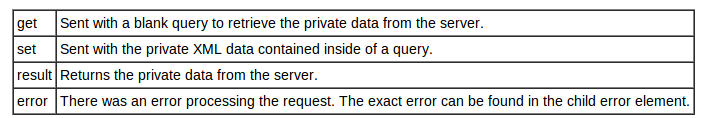
\includegraphics[scale=0.9]{images/xep0049Queries.png}   
		\caption[ Description of Acceptable Methods]{Description of Acceptable Methods}   
		\end{figure}
	\subsubsection{Elements}
	The root element of this namespace is query. At least one child element with a proper namespace must be included; otherwise the server must respond with a "Not Acceptable" error. A client must not query for more than one namespace in a single IQ get request. However, an IQ set or result may contain multiple elements qualified by the same namespace~\ref{client_save}.
    \begin{lstlisting}[label=client_save,caption=Client Stores Private Data]
	CLIENT:
	<iq type="set" id="1001">
	  <query xmlns="jabber:iq:private">
	    <exodus xmlns="exodus:prefs">
	      <defaultnick>Alice</defaultnick>
	    </exodus>
	  </query>
	</iq>

	SERVER:
	<iq type="result"
	    from="alice@likepro.co/"
	    to="alice@likepro.co/"
	    id="1001"/>
    \end{lstlisting}

     \begin{lstlisting}[label=client_load,caption=Client Retrieves Private Data]
		CLIENT:
		<iq type="get" id="1001">
		  <query xmlns="jabber:iq:private">
		    <exodus xmlns="exodus:prefs"/>
		  </query>
		</iq>

		SERVER:
		<iq type="result"
		    from="alice@likepro.co/"
		    to="alice@likepro.co/"
		    id="1001">
		  <query xmlns="jabber:iq:private">
		    <exodus xmlns="exodus:prefs">
		      <defaultnick>Alice</defaultnick>
		    </exodus>
		  </query>
		</iq>
    \end{lstlisting}

    The message format described above can be made by using two main functions: save(for saving data on the XMPP server) and load(to retrieve saved data from the XMPP server), as shown on the Listing~\ref{save_load_ns}:
	\begin{lstlisting}[label=save_load_ns,caption=Snippet of Save/Load preferences to a private namespace]
	      	save: function (property) {
	            xmpp.connection.private.set(property, property + ":ns", user[property], function (data) {
	                    console.log(property + " saved: ", data);
	                },
	                console.log);
	        },
	        load: function (property) {
	            xmpp.connection.private.get(property, property + ":ns", function (data) {
	                    user[property] = data != undefined ? data : [];
	                    if (property == 'subscriptions') {
	                        for (var i = 0; i < user.subscriptions.length; i++) {
	                            xmpp.subscribe(user.subscriptions[i]);
	                        }
	                    }
	                    $rootScope.$apply();
	                },
	        }
	\end{lstlisting}


%%%%%%%%%%%%%%%%%%%%%%%%%%%%%%%%%%%%%%%%%EVALUATION%%%%%%%%%%%%%%%%%%%%%%%%%%%%%%%%%%%%%%%%%%%%%%%%%%%%%%%%%%%%%%%%%%%%
\section{Evaluation}
Evaluation are done as a proof of concept by demonstrating a scenario of distributed XMPP-driven web site accessing data from a hardware and software sensors. Where as software sensor was taken a bot, which periodically sends some IT news in a text format. And as a hardware sensor was used a temperature sensor from university. To the prototype was given a name: SensDash(Sensor Dashboard). Temperature sensor was provided as a testing environment in scope of ACDSee project, together with TU Dresden, BTU Cottbus - Senftenberg and RWTH Aachen University. It locates in the room INF3084, Faculty of Information Technology, Chair of Computer Science. The sensor part represents a class of low-cost, high-performance sensors. It is implemented using a commercially available Raspberry Pi single-board computer with an affiliated USB thermometer and automatic WLAN and XMPP connections to a sensor MUC room established at boot time. Everything concerning sensor are installed on Mobilis server. According to the system architecture on the Figure 5.10, everything concerning sensor data are assumed implemented on a DataHub. Which has pre-installed XMPP server supporting MUC rooms, each carry a description field which qualifies them as sensor MUC rooms. The temperature sensor itself is a Data Source 1 and Data Source 2 respectively is a software sensor  presented on the Figure 5.10.
        \begin{figure}[!ht]
		\centering
		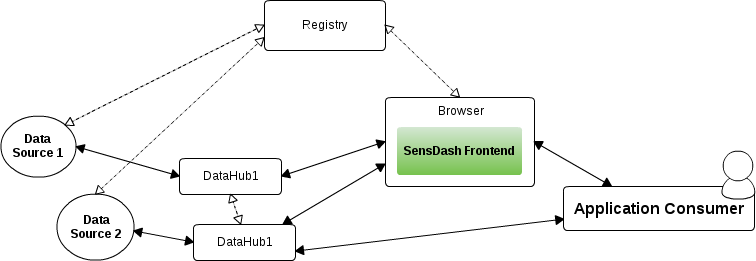
\includegraphics[scale=0.6]{images/UseCaseScheme1.png}   
		\caption[Use Case System Architecture Scheme]{System Architecture Scheme}                         
		\end{figure}

The temperature sensor available from a MUC room: xmpp://inf3084@conference.mobilis-dev.inf.tu-dresden.de and has the next JSON description(Listing~\ref{json_sensor}):
	\begin{lstlisting}[label=json_sensor,caption=JSON Description Format]
{
    "sensormuc": {
        "type": "AMBIENT_TEMPERATURE",
        "format": "short",
        "location": {
            "countryCode": "DE",
            "cityName": "Cottbus",
            "latitude": 51.076834,
            "longitude": 13.772586
        }
    }
}
	\end{lstlisting}
Firstly it has to be registered in the Sensor Registry with an unique id and fulfill the attributes defined in JSON Registry standard accordingly. Since in scope of Master Thesis neither in scope of ACDSee project not included to implement automative Registry, where sensor have to be registered, metadata describing temperature sensor was added manually. The full example of metadata existed in Registry can be found in Appendix A, and the Listing~\ref{sensor_registry} below presents only main charactristics, defined as attribute:
	\begin{lstlisting}[label=sensor_registry,caption=JSON Description Format]
	[
     {
            "id": "30",
            "title": "Ambient Temperature INF3084",
            "availability": true,
            "description": "DSE students receive an opportunity to get current outdoor temperature in Dresden Momsenstr.20. This sensor provides temperature updates with 5-second frequency and represents a class of low-cost, high-performance sensors. It is implemented using a commercially available Raspberry Pi single-board computer with an affiliated USB thermometer and automatic WLAN and XMPP connections to a sensor MUC room established at boot time.",
            "sla": "Sensor resolution is 0.5 C, measurements taken every 10 seconds. Uptime 95% from 6:00 till 22:00.",
            "sla_last_update":"1395005996",
            "access": "private",
            "provider_name": "Provider TU Dresden",
            "location": "Dresden",
            "end_points": [
                {
                    "type": "muc",
                    "priority": "main",
                    "name": "xmpp://inf3084@conference.mobilis-dev.inf.tu-dresden.de",
                    "pwd": null
                },
                {
                    "type": "muc",
                    "priority": "alternative",
                    "name": "xmpp://inf3086@conference.mobilis-dev.inf.tu-dresden.de",
                    "pwd": null
                },
                {
                    "type": "muc",
                    "priority": "optional",
                    "name": "xmpp://inf3087@conference.mobilis-dev.inf.tu-dresden.de",
                    "pwd": null
                }

            ],
            "type": "chart"
        }
]
	\end{lstlisting}
Demonstration of activity scenario was made by using 3d party user which is application consumer developer. His name Max and he has to create specific mobile application. A sa result, firstly he needs to define which sensors to use and how to retrieve an info from it. 
\subsection{Use Case Scenario}

\textbf{Step 1:} In order to find necessary sensor, explore description and data provided by it, Max has to sign in into the SensDash by using peronal JID and password, received from an dministrator of a SensDash(Figure 5.11).
\begin{figure}[!ht]
\centering
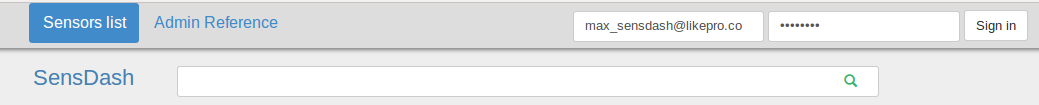
\includegraphics[scale=0.6]{Screenshots/signIn.png}   
\caption[Log in to the SensDash]{Log in to the SensDash}                         
\end{figure}

\textbf{Step 2:} After successfully passing authorisation, Max can start searching necessary sensors. By using search field, he can enter the one of the key word which is clearly define purpose or type of a sensor, and immediately list of sensors will be sorted based on his search input. To get more detailed information about sensor he clicks on the field of sensor. In a new popup window(Figure 5.12), and if to be more precise, it is a new tool, called modal. In the appeared modal, user can get a detailed description about sensor, e.g. : SLA, location, provider, preview, development details such as end-points quantity, end-point configuration, administrator name and of course more sophisticated description. This information gives an overview of what type of data provided by data source. 
\begin{figure}[!ht]
\centering
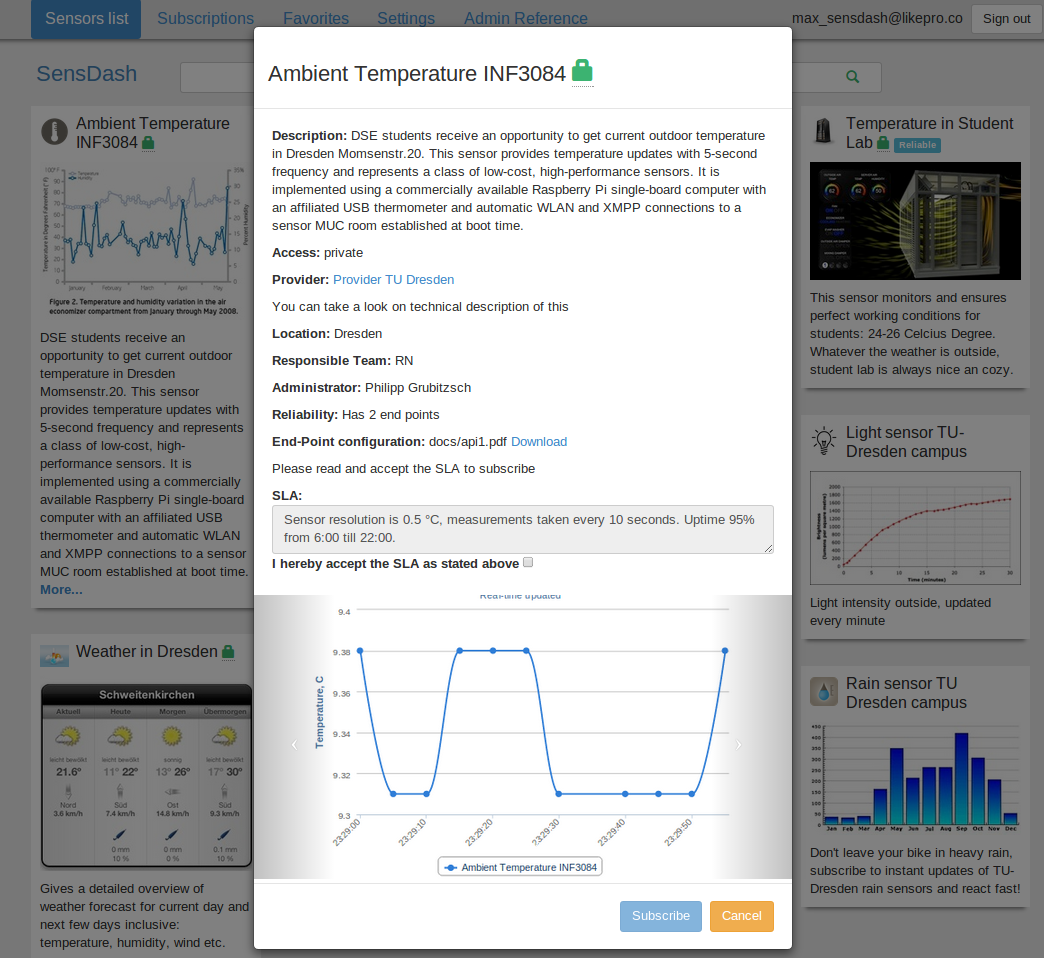
\includegraphics[scale=0.6]{Screenshots/UseCaseWelcome.png}   
\caption[Personal Modal of a Sensor]{Personal Modal of a Sensor}                         
\end{figure}
 
 In case of ambient temperature INF3084, Max can explore predefined preview, which consists graph of provided temperature, data values and it's frequency, security level and relialability. In case of software sensor it can be sample of news feed, provided by sensor. 

\begin{figure}[!ht]
\centering
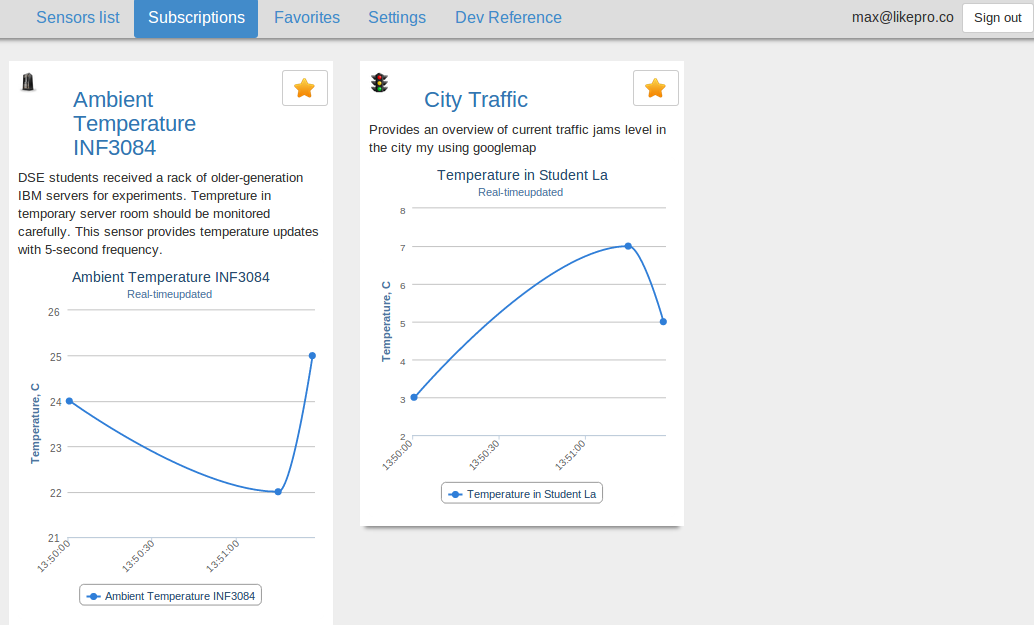
\includegraphics[scale=0.6]{Screenshots/UseCaseScreenshot4.png}   
\caption[Personal Subscribed Sensor]{Subscriptions list}                         
\end{figure}
\textbf{Step 3:} Since the ambient temperature sensor is a private sensor, Max has to accept SLA before getting a real-time data from it. In contrast to temperature sensor, a software sensor - IT news feed has a public access, thus, Max doesn't need to accept any SLA in order to see real-time data provided by this sensor. The common rule, which is applied to every sensor independently from its access type(public or private) is to subscribe to it. In such a way, all sensors, to which Max has subscribed will appear in the next tab called "Subscriptions". And as soon as new data become available SensDash retrieve it in this (Figure 5.13). Also, by using Subscriptions Tab and icon "star" in a right corner, become possible to add subscribed sensor to the Favorites. After clicking on the icon of favorites, sensor information will appear in a list of favorites in Favorites Tab.

\textbf{Step 4:} To get info about personal account Max have to use Settings Tab. Where exists personal profile settings(Figure 5.14). 
\begin{figure}[!ht]
\centering
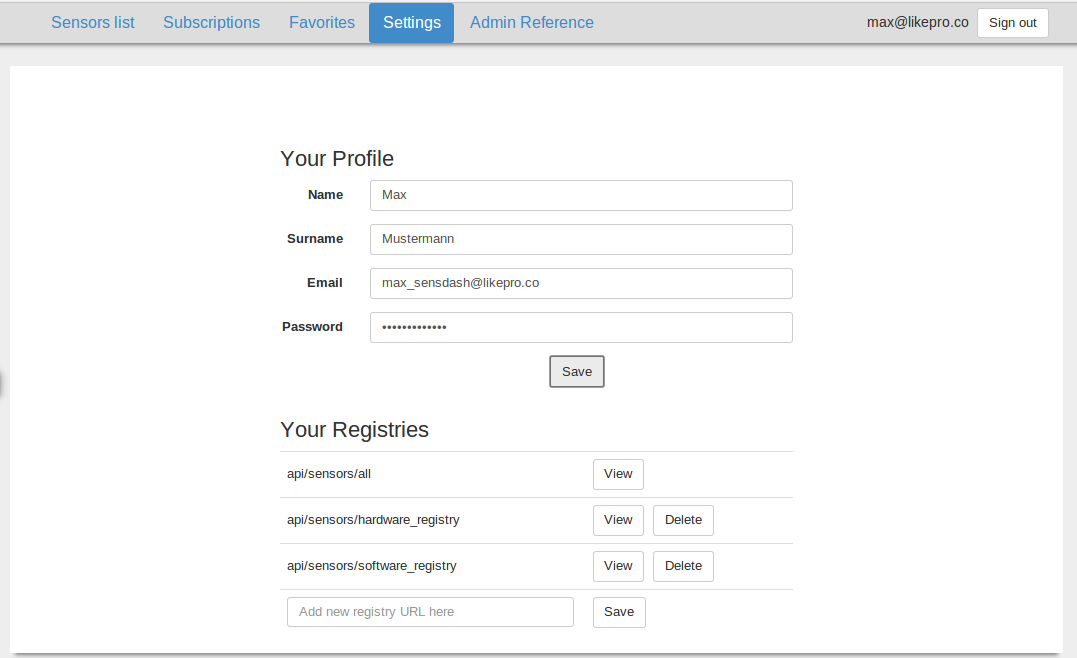
\includegraphics[scale=0.6]{Screenshots/UseCaseSettings.png}   
\caption[Settings Tab]{Settings Tab}                         
\end{figure}

\textbf{Step 5:} As a developer, Max might be interested in technical details of sensor data retieval process, e.g. API references, end-point configuration, sensor data format, interface and system architecture in order to interconnect with backend directly. So Max has to go to the Admin References Tab(Figure 5.15), where he can find all available implementation detailes of a frontend itself, protocol and its extensions realization and system architecture. 
\begin{figure}[!ht]
\centering
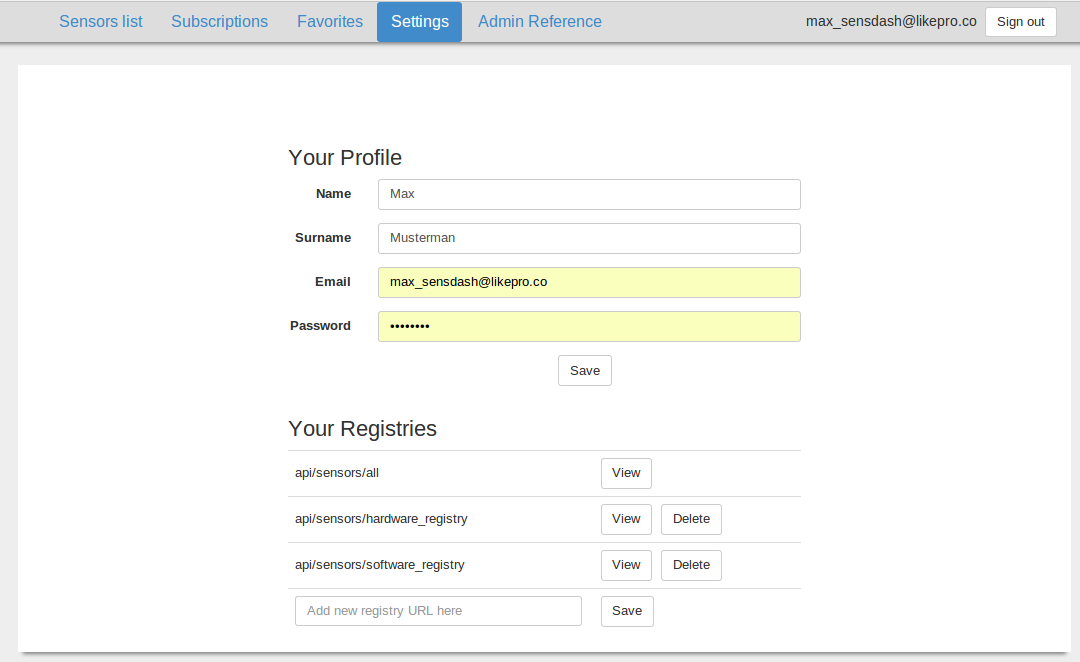
\includegraphics[scale=0.6]{Screenshots/UseCaseScreenshot6.png}   
\caption[Administrator Tab]{Administrator Tab}                         
\end{figure}

\subsection{SensDash Implementation}
After real example of SensDash usage was described in the previous section, needs to be clarified the concept overflow together with used and implemented XMPP extensions.

\textbf{Log In}to the system can be possible only with valid JID and password, which have to be registered within any possible XMPP server. Since XMPP network structured very similar to DNS, doens't metter where registered JID. The only one important thing is to know which XMPP server carry on MUC room. Firstly, user credentials validated by input type on frontend side and only than sended to the backend. Once XMPP server authorize the user, JID and password are saved in a browser by using cookies. So the next time when the user will open abrowser URL of a SensDash, cookies will automatically log him/her into the system. 

\textbf{Preferences Saving} are done by using XEP0049 and stored on the XMPP server. When a user sign in to the system first time, application logic creates fully empty account with no subscriptions and favorites. Once a user subscribes to any resource, this resource automatically appear on Subscriptions Tab and added to the subscriptions map. The same for favorites and Favorite Tab, but favorites, due to simple structure are saved in a simple favorites array. It means that system has saved this preferences on XMPP server by using one of the extension called XEP0049, based on private space for every JID without interconnection with backend. Next time when user will log in to the system, all saved subscriptions and favorites will be loaded in the meanwhile and appear in corresponding tabs. An example subscriptions map and favorites array for Max are presented in Appendix B.

\textbf{Functional characteristic of a sensor}
\newline
In the section 4.4 was clarified 3 main characteristics which acquire sensor based on a system architecture. Since realization of a Data Hub fully rely on a backend, but in proposed evaluation was used XMPP server, become possible to differentiate security, reliability and performance level based only on a server configuration. Where every end-point is a MUC chat room(Figure 5.16). 
\begin{figure}[!ht]
\centering
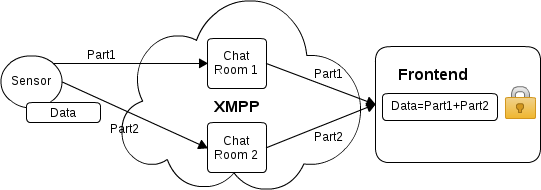
\includegraphics[scale=0.6]{images/security.png}   
\caption[Security]{Data secure transfer using Chat Rooms}                         
\end{figure}
Application logic calculate automatically number of available end-points for every sensor, based on Registry info and shows it on the main page as shown above on the Figure 5.17. The rules of how was calculated the security level or reliability are described in the Section 4.4, Subsection "Sensor Functional Characteristics".
\newline
\begin{figure}[!ht]
\centering
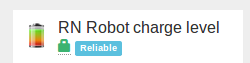
\includegraphics[scale=1.0]{Screenshots/Icons.png}   
\caption[GUI identification of security and reliability level]{GUI identification of security and reliability level}    
\end{figure}

\textbf{Search Bar} is made by using only frontend, as one of the feature of the AngularJS. It makes sorting of an graphical object through the all existed titles of a data source. It is fast and very straightforward in use. 

\textbf{Data Streaming} is the point where Data Hub as a part of a backend come into a picture. All data streaming works through XMPP extensions called XEP0049(MUC) or XEP0045(MUC). In presented example with ambient temprature in INF3084 was used MUC for retrieving real-time data throug the BOSH. Since generic frontend supposed to support all possible approaches, it also provides realization for PubSub(XEP0060). By using Strophe.js as a client-side web-based library was made refactoring according to skeleton defined by AngularJS. 
\newline
The SensDash logic builded on top of AngularJS skeleton(Appendix C). By using two-way data binding, aggregation and presentation of a sensor metadatadata was done by using factory pattern. Together with creation of a sensor entity as a graphical object, all handlers, functionality and interconnection protocol also created for every object accrodnigly, based on abstract methods. Such a general manipulation of objects makes possible to loosely couple code and object. All sensors metadata will be automatically parsed from Sensor Registry and presented on a SensDash always in the same way. Everything done in runtime, such that if a new sensor registers itself in Registry it will appear as soon as user reload the page. 

\section{Summary}
This chapter presents details of implementation of the generic frontend concept. At first, choosen tools and development environment were presented: jQuery, HTML5, CSS as a programming language, AngularJS together with Bootstrap to interconnect application logic with XMPP interface standard and Strophe.js was picked to implement the XMPP mechanism and it's extensions. Web API was defined and afterwards used to retrieve from the Registry all available sensors by sending direct HTTP GET request. Authentification and data streaming from a web browser and XMPP server was made by using XMPP BOSH standard and XEP0049, XEP0045 extensions, based on Strophe.js and part of the was refectored as skeleton for AngularJS. 

All used technologies, protocols, libraries and methodologies was gathered together in order to realize working prototype. A summary overview of all described above compunents and tools are shown on the Figure 5.19
\begin{figure}[!ht]
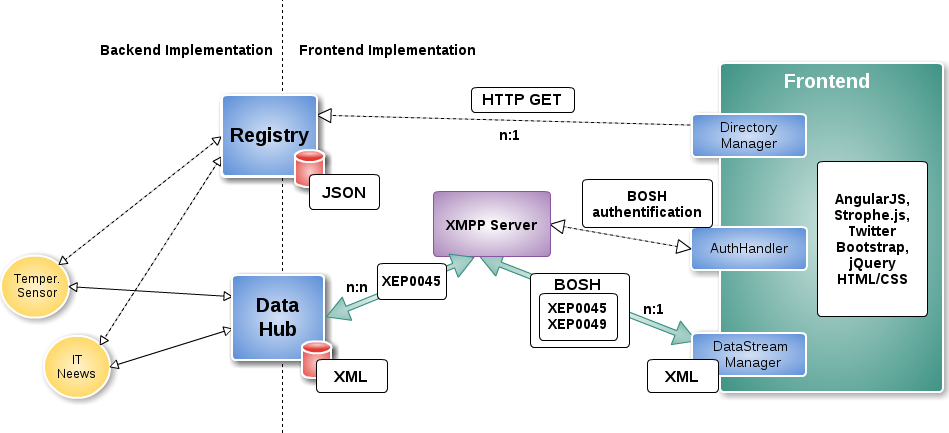
\includegraphics[scale=0.5]{images/ch5Summary.png}   
\caption[Implementation Architecture]{Implementation Architecture}                         
\end{figure}
Was presented the convinsing scenario based on ambient temperature sensor from room INF3084 and consumer application developer's requirements.

